\documentclass[a4paper,11pt]{article}

\title{Exercise: Importing Figures}
\author{Stu Dent}

\usepackage{amsmath, amssymb, amsfonts}

\usepackage{amsthm}
\theoremstyle{plain}
\newtheorem*{thmTaylorLagrangeRemainder}{Taylor's Theorem with Lagrange's Remainder}

\usepackage{graphicx}
\graphicspath{{./imgs/}}
\usepackage{subcaption}

\usepackage[numbers]{natbib}
\bibliographystyle{plainnat}
\usepackage{cite}

\usepackage{url}

\begin{document}
\maketitle

\section*{Lagrange's Theorem}

\begin{figure}[hbtp]
	\centering
	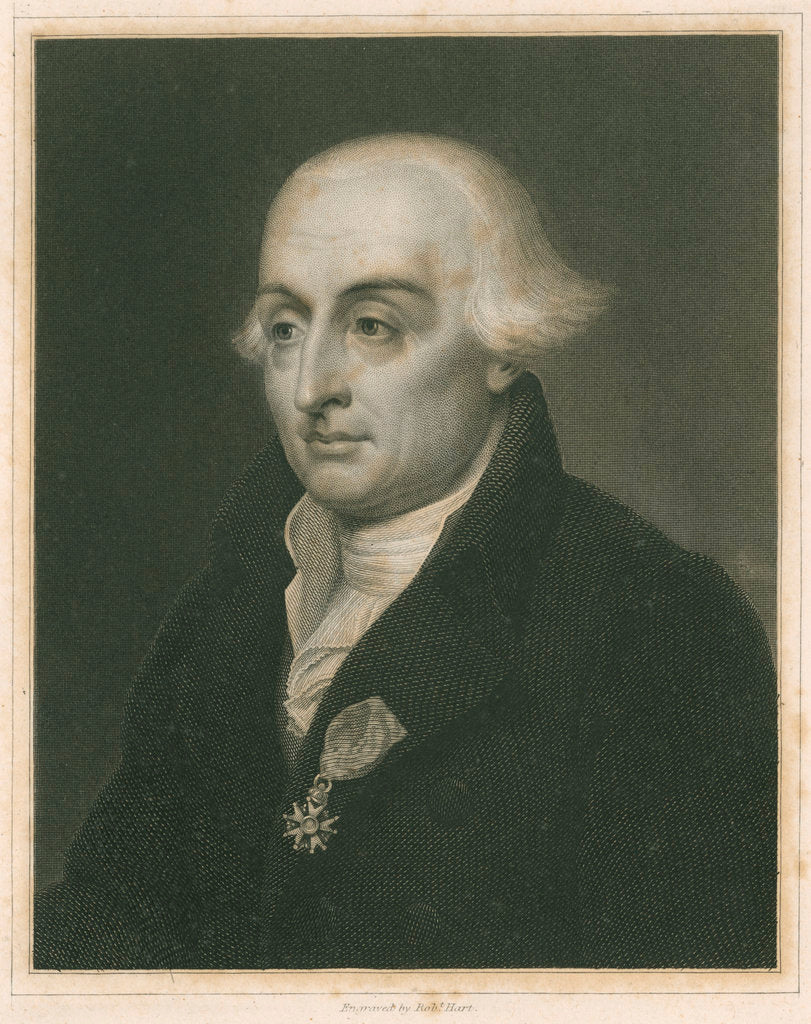
\includegraphics[width=2.5in]{lagrange-portrait.jpg}
	\caption{Portrait of Joseph-Louis Lagrange\protect\footnotemark}
	\label{fig:lagrange-portrait}
\end{figure}
\footnotetext{Portrait by Robert Hart, taken from \citep{hart-lagrange-portrait}}

Lagrange, pictured in Figure~\ref{fig:lagrange-portrait}, was an Italian-French mathematician and astronomer who made significant contributions to the fields of analysis, number theory, and both classical and celestial mechanics. Interestingly, Lagrange himself did not prove Lagrange's~Theorem --- this was done by Jordan in 1861. However, the theorem was named after Lagrange because he states a specialises application of it to polynomials in his article \textit{R{\'e}flexions sur la r{\'e}solution alg{\'e}brique des {\'e}quations}\citep{langrange-1770-reflexions}.

\section*{Taylor's Theorem}

Indeed, many A-level students will be familiar with writing Taylor expansions of nice functions such as
\begin{equation}\label{eqn:taylor-expansion-sin}
\sin(x) = x - \frac 13 x^3 + \frac 15 x^5 + \cdots
\end{equation}
and they may even be familiar with the generalisation of this
\begin{align*}
f(x) &= f(x_0) + f'(a)(x - x_0) + \frac 12 f''(x_0)(x - a)^2 + \frac 1{3!} f'''(a)(x - x_0)^3 + \cdots \\
&= \sum_{k=0}^\infty \frac{1}{k!} f^{(k)}(x_0) (x - x_0)^k.
\end{align*}

Certainly these expansions seem to work for all nice functions encountered by A-level students. However, these expansions need more care. There are important questions to address such as whether the pattern can continue forever, and if so whether it converges, and then if so, whether it converges to the claimed function. The first of these questions is relatively easy to address. For the series to exist, we must require that $f^{(k)}(x_0)$ exists for all $k \in \mathbb{N}$ and hence that $f$ needs to be $C^\infty$ in some neighbourhood of $x_0$.

But even if we relax this criteria, we can extend the Mean Value Theorem naturally to work for higher derivatives which allows us to make powerful approximations of functions using polynomials. There are many ways that mathematicians can measure the error in these approximations and possibly the easiest to remember is that associated with Lagrange as the remainder term looks similar to the next term we might have expected.

\begin{thmTaylorLagrangeRemainder}
Suppose that $f \colon [x, x_0] \to \mathbb{R}$ is $n + 1$ times differentiable on $(x, x_0)$ and that its $n$\textsuperscript{th} derivative $f^{(n)}$ is continuous on $[x, x_0)$. Then there exists some $\xi \in (x, x_0)$ which satisfies \[
f(x) = \sum_{k=0}^n \frac 1{k!} f^{(k)}(x_0) (x - x_0)^k + R^n(x)
\]
where the remainder term $R_n(x)$, the so-called Lagrange remainder is given by \[
R_n(x) = f^{(n+1)}(\xi) (x - x_0)^{n+1}.
\]
\end{thmTaylorLagrangeRemainder}

Figure~\ref{fig:taylor-polynomials-of-sin} illustrates this concept for the sine function about the point $x_0 = 0$. The figure allows us to visualise how quickly these polynomials become increasingly more accurate as the degree $n$ of the polynomials increase. This suggests that the Lagrange remainder $R_n(x)$ here should tend to zero as $n$ tends to infinity.

\begin{figure}[hbtp]
	\begin{subfigure}{0.5\textwidth}
		\centering
		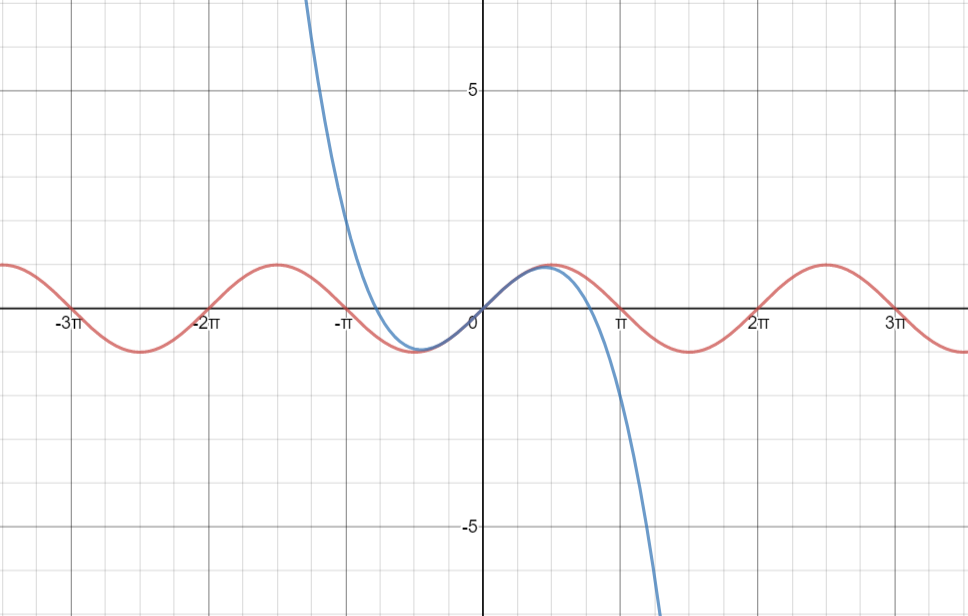
\includegraphics[width=0.9\textwidth]{taylor1}
		\caption{Degree $n=1$}
	\end{subfigure}
	\begin{subfigure}{0.5\textwidth}
		\centering
		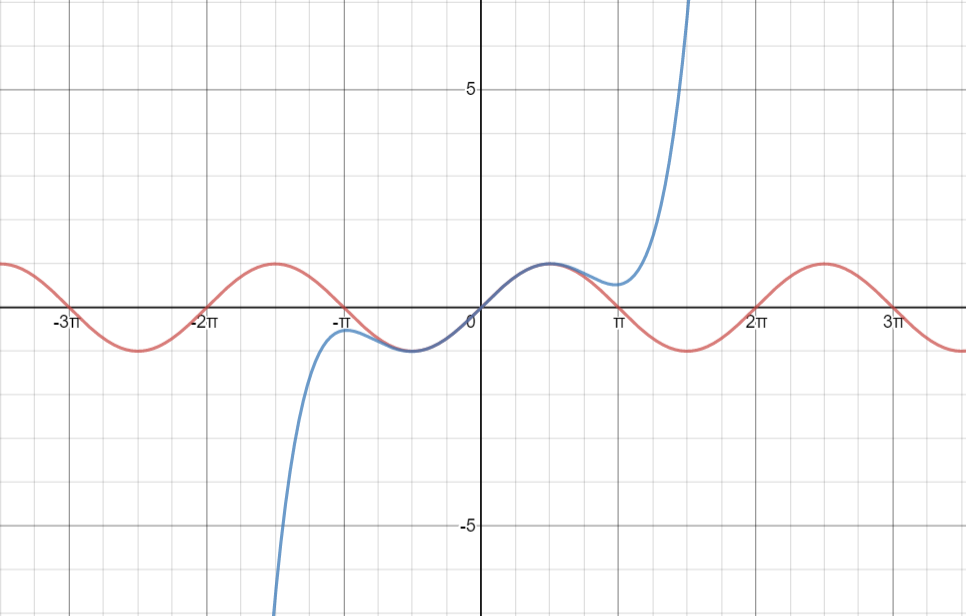
\includegraphics[width=0.9\textwidth]{taylor2}
		\caption{Degree $n=2$}
	\end{subfigure}

	\begin{subfigure}{0.5\textwidth}
		\centering
		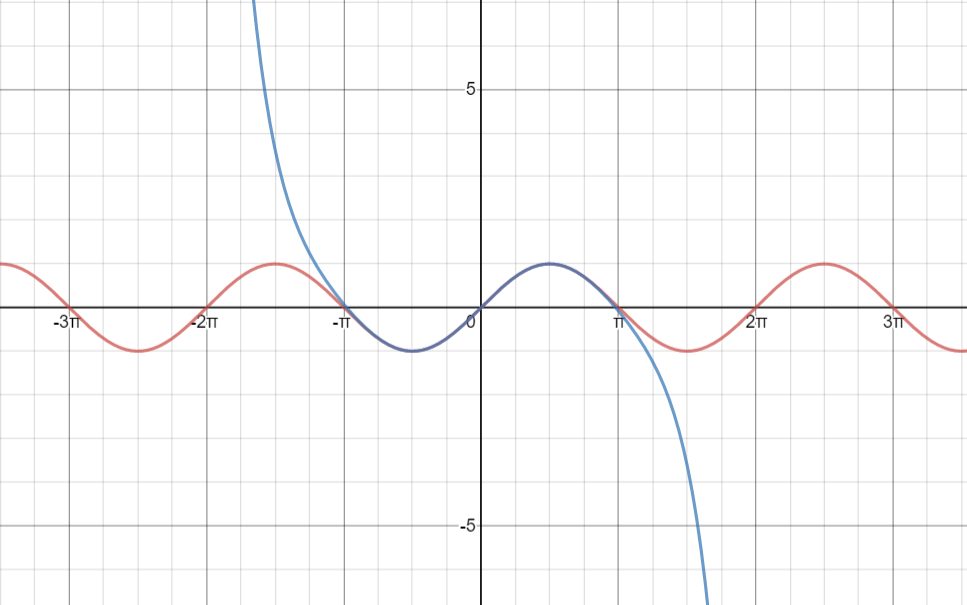
\includegraphics[width=0.9\textwidth]{taylor3}
		\caption{Degree $n=3$}
	\end{subfigure}
	\begin{subfigure}{0.5\textwidth}
		\centering
		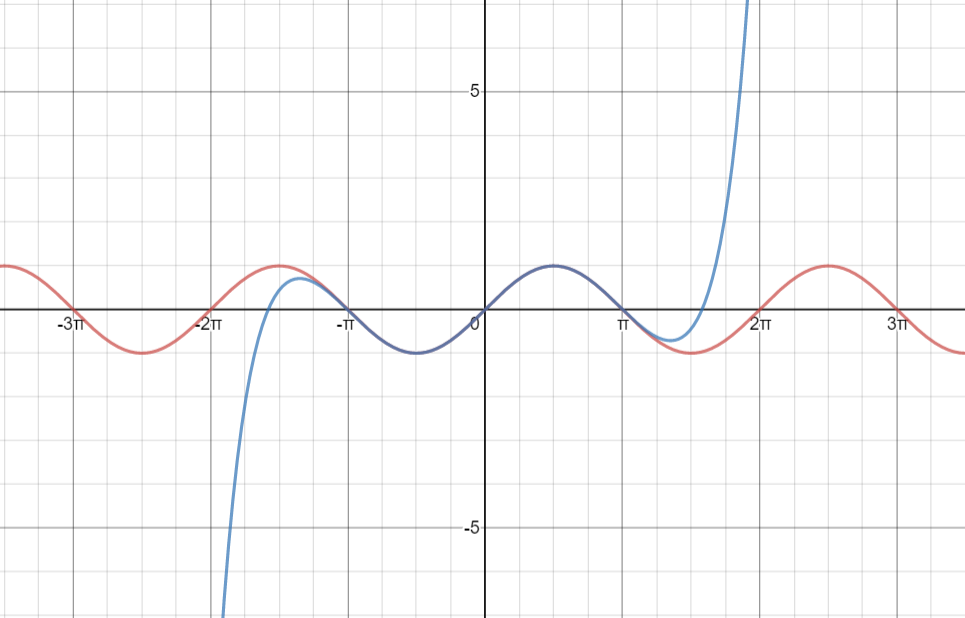
\includegraphics[width=0.9\textwidth]{taylor4}
		\caption{Degree $n=4$}
	\end{subfigure}

	\begin{subfigure}{0.5\textwidth}
		\centering
		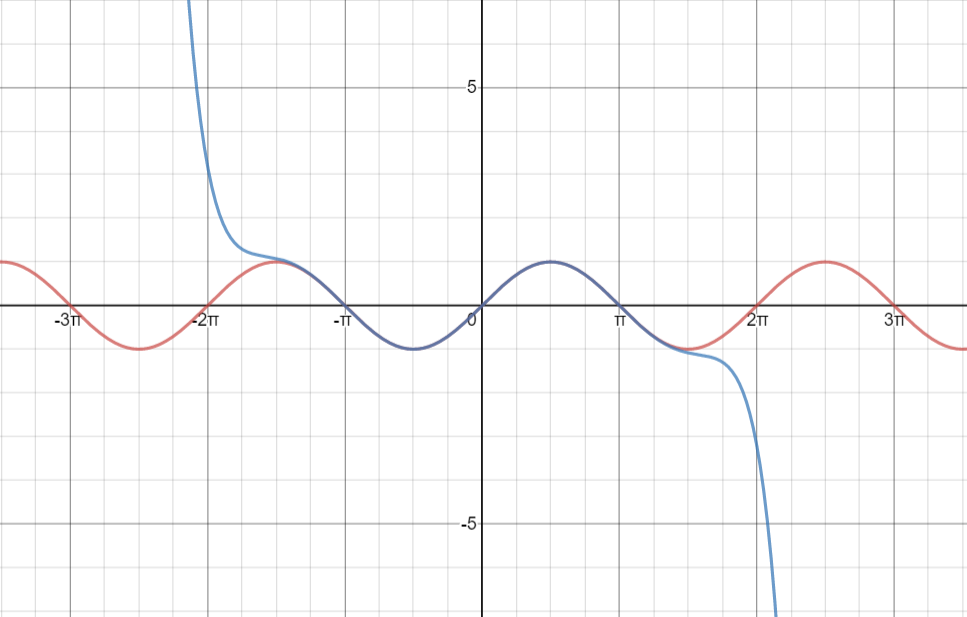
\includegraphics[width=0.9\textwidth]{taylor5}
		\caption{Degree $n=5$}
	\end{subfigure}
	\begin{subfigure}{0.5\textwidth}
		\centering
		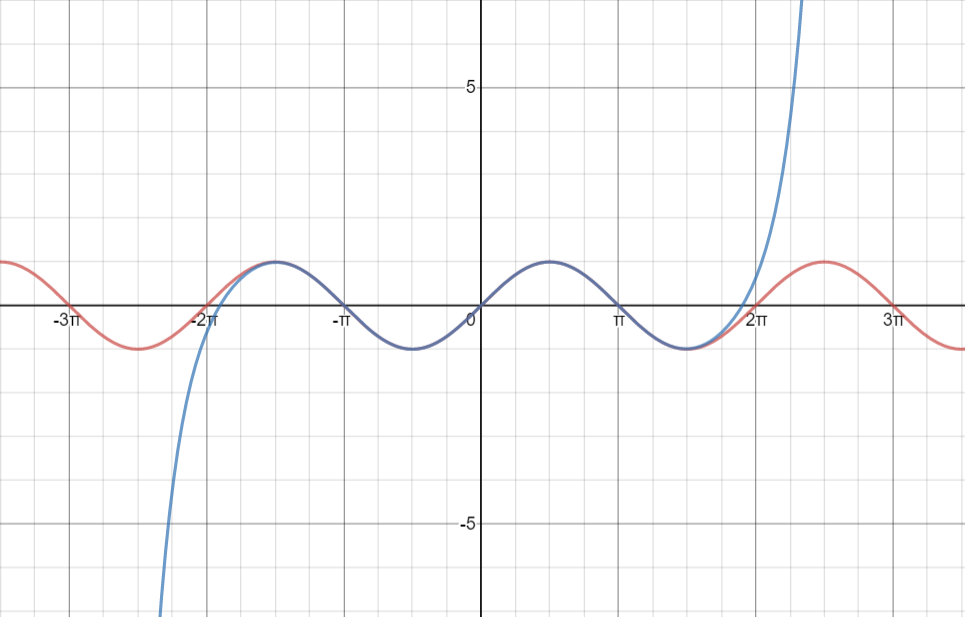
\includegraphics[width=0.9\textwidth]{taylor6}
		\caption{Degree $n=6$}
	\end{subfigure}

	\caption{Taylor polynomials of varying degree $N$ (blue) of the function $\sin$ (red)}
	\label{fig:taylor-polynomials-of-sin}
\end{figure}

\bibliography{main}

\end{document}
